\documentclass[12pt,letterpaper]{article}

\usepackage[hmargin=1in,bottom=1in,top=1in]{geometry}
\usepackage[latin1]{inputenc}
\usepackage{amsmath}
\usepackage{amsfonts}
\usepackage{amssymb}
\usepackage{graphicx}
\usepackage{url}
\usepackage[toc,page]{appendix}
\usepackage{setspace}
\usepackage{pdfpages}

\usepackage{ulem}
\normalem

% push footnotes to the bottom of the page unconditionally
\usepackage[bottom]{footmisc}

\bibliographystyle{IEEEtran}

\setlength{\parindent}{0in}
\setlength{\parskip}{1.0 \baselineskip}
\setlength{\footnotesep}{1.0 \baselineskip}
\setlength{\skip\footins}{2.0 \baselineskip}

\newenvironment{enumeration}{
	\setlength{\topsep}{0.0pt}
	\setlength{\partopsep}{0pt}
	\setlength{\parskip}{0pt}
	\setlength{\parsep}{0pt}
	\begin{enumerate}
		\setlength{\itemsep}{0pt}}
	{\end{enumerate}}

\newenvironment{itemlist}{
	\setlength{\topsep}{0pt}
	\setlength{\partopsep}{0pt}
	\setlength{\parskip}{0pt}
	\setlength{\parsep}{0pt}
	\begin{itemize}
		\setlength{\itemsep}{0pt}}
	{\end{itemize}}

\newcommand{\sectref}[1]{Section \ref{#1}}
\newcommand{\figref}[1]{Figure \ref{#1}}
\newcommand{\tableref}[1]{Table \ref{#1}}

\begin{document}

\begin{titlepage}
\begin{center}


\includegraphics[scale=1.0]{ecelogo.png}

\vspace{1 \baselineskip}

\textsc{
\Large University of Toronto\\
\large Department of Electrical and Computer Engineering \\
\large ECE496 Design Project
}

\vspace{2 \baselineskip}

{\Large \bfseries Virtual FPGA fabrics} \\
{\Large \bfseries Implementation of a Virtual FPGA Architecture}

\vspace{2 \baselineskip}

{\large \bfseries Individual Progress Report} \\
%{\large \bfseries Final Version}

\vspace{2 \baselineskip}

{\large January 17, 2012}

\vfill

\begin{tabular*}{4in}{l @{\extracolsep{\fill}} l}
\textbf{Keyi Shi} & \texttt{keyi.shi@utoronto.ca} \\ & \\
\emph{Project ID:} & 2011017 \\
\emph{Supervisor:} & Jason Anderson \\
\emph{Administrator:} & Ross Gillett \\
\emph{Section:} & \#7 \\
\end{tabular*}

\end{center}
\end{titlepage}

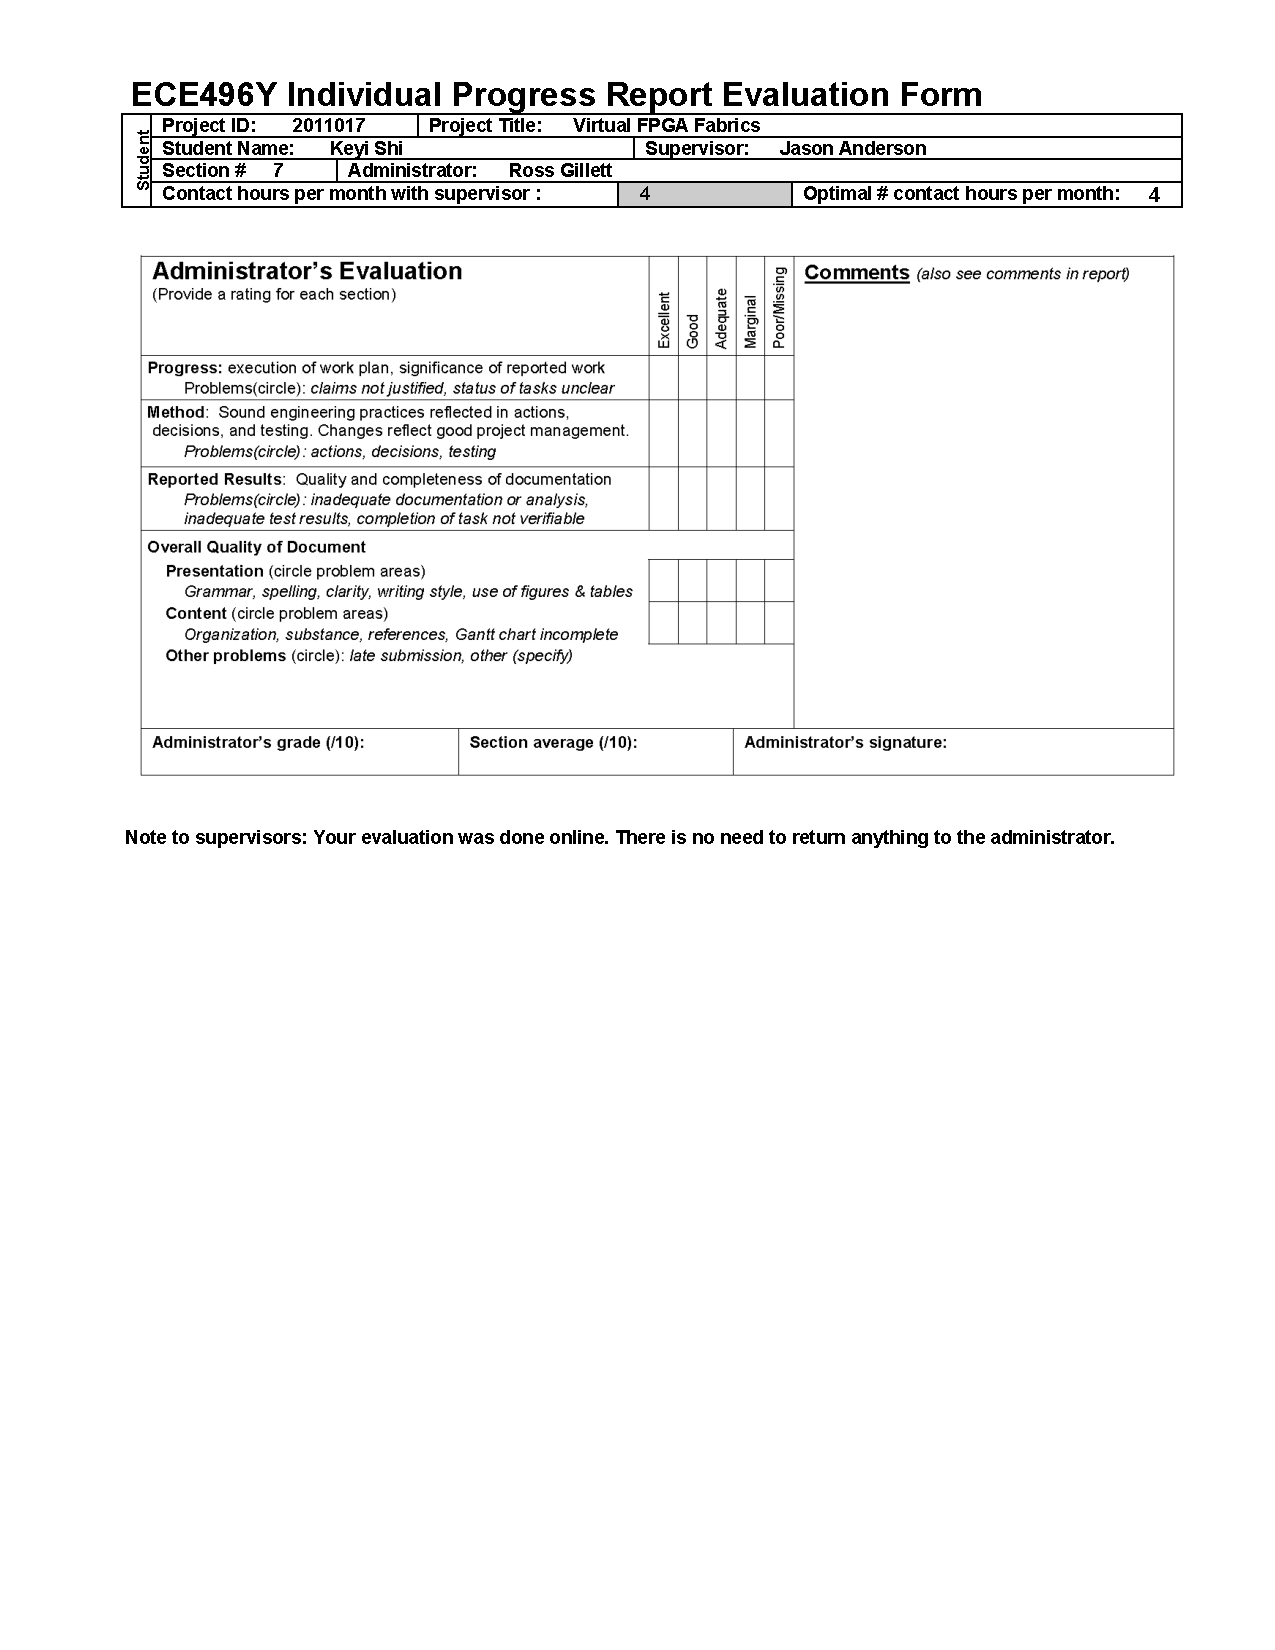
\includepdf{cover-sheet-keyi.pdf}

\onehalfspace

\thispagestyle{empty}
\section*{Executive Summary}

The project overall has progressed smoothly to the overlay building stage, and we are now attempting communicate between the overlay and a VPR-generated bitstream.

I have worked exclusively on the hardware side of this project, building and testing the basic building blocks of the overlay, as well as generating the overlay itself. 
My current goals are to work with Neil to get the overlay and VPR bitstream generator working together, as this is the next crucial step in the project.

We have extended our schedule and deadlines from our initial proposal.
We intentionally budgeted a large amount of spare time at the end of the term to be used on possible complications and bugs in the project, as the nature of this projects requires extensive debugging in order to get all of the components to function together.

Our overlay design turned out to be quite resource consuming, and as it stands we cannot fit as large a virtual FPGA onto a commercial board as we would have liked.
This was a risk identified in the proposal, but we believe we can still produce an overlay large enough to house meaningful circuits for demonstration and proof-of-concept purposes.
If there is extra time left at the end of the project, we may attempt to improve the efficiency of our overlay design.

\pagebreak
\pagenumbering{arabic}

\section{Individual Progress and Contributions}

The following table is an overview of my contributions to the project.
An updated Gantt chart may be found in Appendix A.

\begin{tabular}{|l|l|l|l|l|l|l|}
\hline
\textbf{Task title} & \textbf{Category} & \textbf{Status} & \textbf{Original date} & \textbf{New date} \\ \hline
\hline
1. Basic virtual overlay modules & hardware & completed & Aug-Oct 15 & Aug-Nov 2 \\ \hline
2. Complete overlay design & hardware & debugging & Oct 15-Jan 15 & Nov2-Jan 20 \\ \hline
3. Stress-testing and improvement & testing & not started & Dec 15-Apr 1 & Jan 15-Apr 1 \\ \hline
\end{tabular}


\section{Information on individual Milestones}

\begin{tabular}{|p{6.4in}|}
\hline
\textbf{1. Basic virtual overlay modules} \\
\emph{Category:} hardware \\
\emph{Original date:} August - October 15 \\
\emph{New date:} August - November 2 \\
\hline
\textbf{Responsibility:} Keyi, Neil \\
I wrote the basic logic element, multiplexer, and switch block. \\
% Neil: UART, logic block, and connection block.
\hline
\textbf{Status:} completed: individual modules are tested and functional according to planned requirements. \\
\hline
\textbf{Actions}
\begin{itemize}
\item I wrote the logic element, multiplexer, and switch block modules.
\item I wrote multi-layer shift-multiplexers for different numbers of inputs.
\item All modules needed to be programmable via a scan chain.
\end{itemize} \\
\hline
\textbf{Decisions} \\
\vspace{-1em}
\begin{itemize}
\item We used the native 32-bit shift registers available on the Virtex 5 board as the building block for our basic modules. The shift registers allowed for the use of a scan chain set up to program all components of the overlay.
\item The different modules required multiplexers of different sizes. In order to simplify coding and save on area, I created a master multiplexer module that adjusted its size to suit the number of inputs required.
\item To keep our project simple and the overhead area down, we decided against giving our switchblock full connectivity.
\item Each module was coded to allow the user to define the number of inputs and outputs from logic blocks, as well as the width of the bus interconnecting the modules.
\end{itemize}
\vspace{-1em} \\
\hline
\textbf{Testing, verification and results} \\
\vspace{-1em}
\begin{itemize}
\item Each module was tested using manually created bitstream files to program different functionalities to ensure correct performance.
Functionality was observed by using on-board switches and LEDs
\end{itemize} 
\vspace{-1em} \\
\hline
\end{tabular}

\begin{tabular}{|p{6.4in}|}
\hline
\textbf{2. Complete overlay design} \\
\emph{Category:} hardware \\
\emph{Original date:} October 15 - January 15 \\
\emph{New date:} November 2 - January 20 \\
\hline
\textbf{Responsibility:} Keyi \\
\hline
\textbf{Status:} debugging \\
The design is complete, but not yet functional with the VPR-generated bitstream.
Further testing is required to determine the source of the problems. \\
\hline
\textbf{Actions} \\
\vspace{-1em}
\begin{itemize}
\item I wrote the overlay grid boundary and interconnects between tiles.
\item I connected the appropriate signals to the inputs and outputs of the overlay.
\end{itemize} 
\vspace{-1em} \\
\hline
\textbf{Decisions}
\begin{itemize}
\item In order to keep track of interconnects and ensure they were placed correctly, we utilized a 2D coordinate system for the overlay grid.
\item We decided to re-use the existing connection block and switch block modules for the boundaries of the overlay in order to save time and keep the code simple.
\item Because of the structure of our connection blocks, the number of outputs per connection block is restricted indirectly by the number of basic logic elements per logic block.
We decided this was an acceptable restriction.
\end{itemize}
\vspace{-1em} \\
\hline
\textbf{Testing, verification and results} \\
\vspace{-1em}
\begin{itemize}
\item Testing is still in progress, and will be more complex than previous hardware testing procedures, as the overlay is much more complex and multi-layered.
\item The resources taken by single tile generated with different parameters has been tested and documented, the results of which are available in Appendix C. The data shows us just how resource-intensive a single tile is currently.
\end{itemize} 
\vspace{-1em} \\
\hline
\end{tabular}

\begin{tabular}{|p{6.4in}|}
\hline
\textbf{3. Stress-testing and improvement} \\
\emph{Category:} testing, hardware \\
\emph{Original date:} December 15 - April \\
\emph{New date:} January 15 - April \\
\hline
\textbf{Responsibility:} Keyi, Neil \\
I will focus on the verification and streamlining of the overlay itself. \\
\hline
\textbf{Status:} not started \\
We will begin extensive verification and improvement once the overlay and bitstream generator work together. \\
\hline
\textbf{Actions} n/a \\
\hline
\textbf{Decisions} n/a \\
\hline
\textbf{Testing, verification and results} \\
\vspace{-1em}
\begin{itemize}
\item Make sure bitstream programs expected circuits onto overlay.
\item Make sure signal routing is always correct.
\item Make sure size of overlay is sufficient.
\item Look into the use of Clos networks to reduce the size of multiplexers.
\end{itemize} 
\vspace{-1em} \\
\hline
\end{tabular}


\section{Progress Assessment}

The majority of the hardware for the project has been coded, and now require extensive testing and debugging to get it working with the bitstream generator.
Once that is done, there are possible improvements to be made to the design to improve the overlay area efficiency on the board.

Overall, the project is progressing well. We have extended our schedule from our initial plans in the proposal, but it was an extremely optimistic schedule and we did budget extra time in the end to allow extensions. As such, we do believe that the project is still well on its way to completion before the design fair.


\pagebreak
\begin{appendices}

\pagebreak

\section{Gantt Chart}
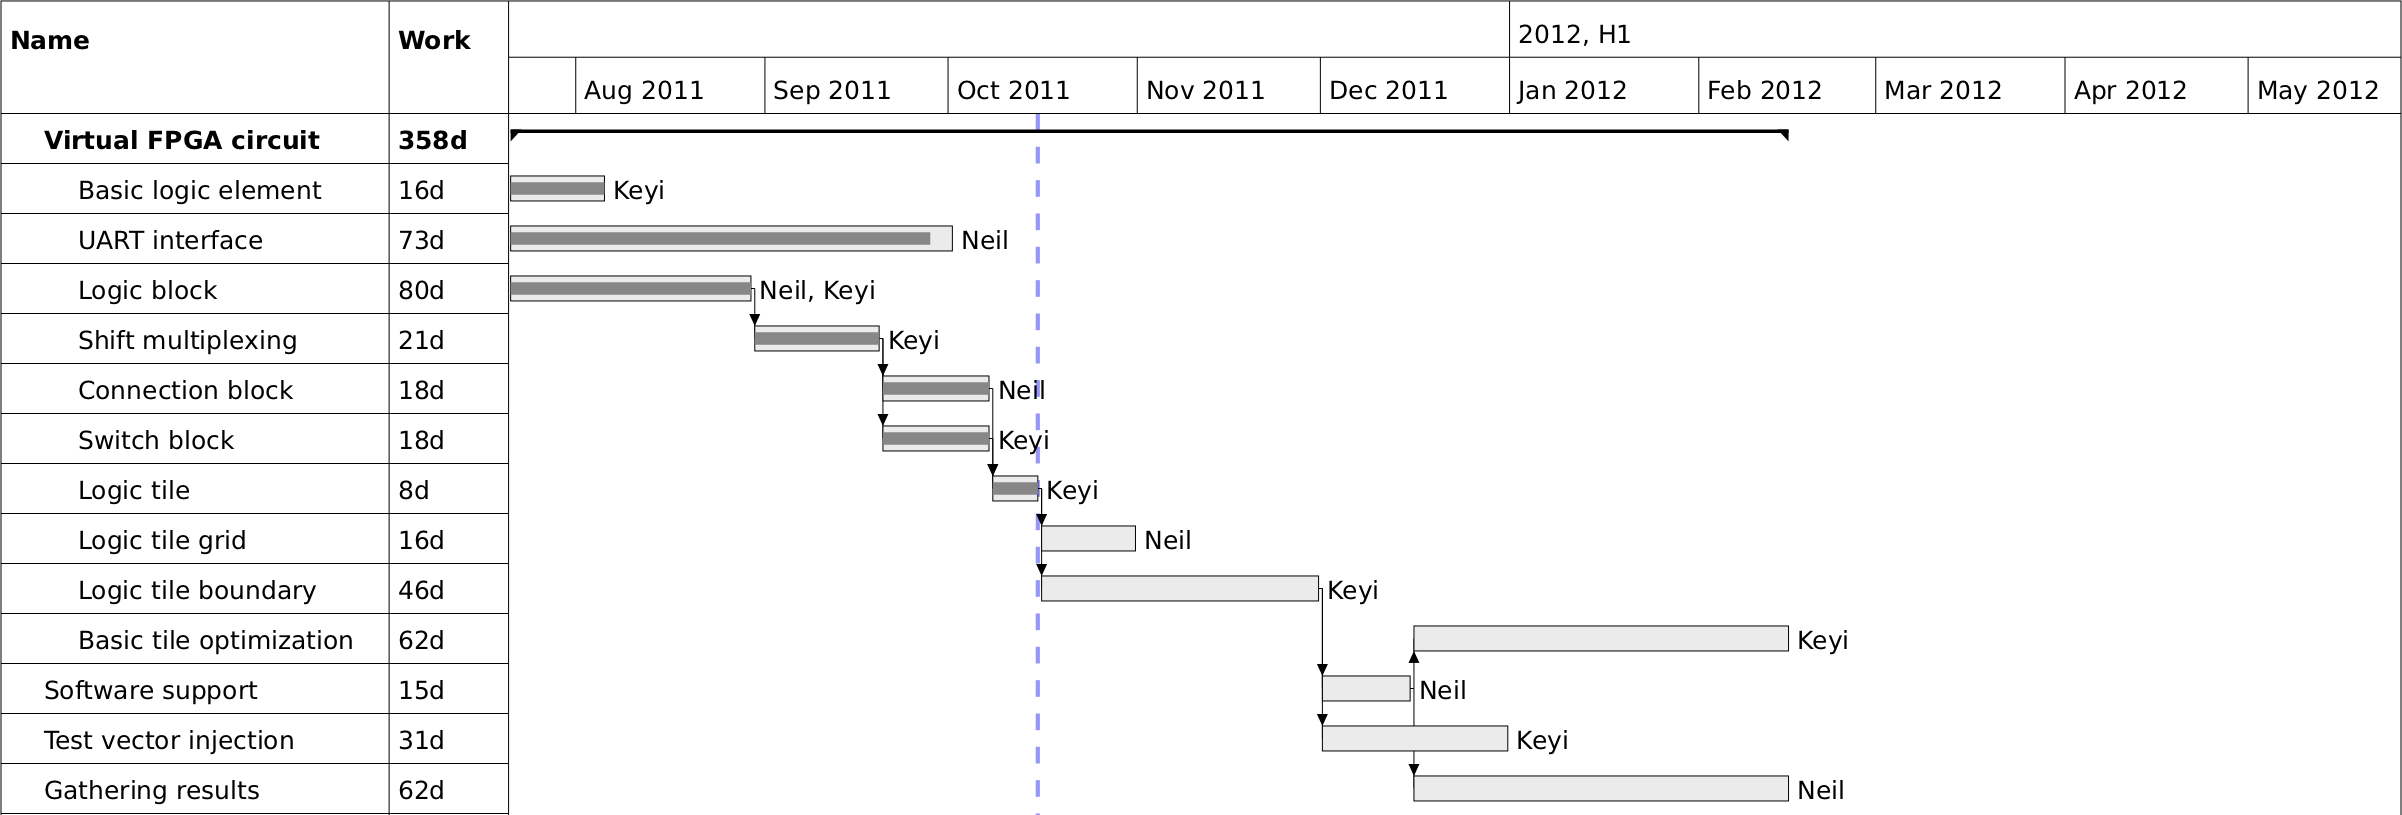
\includegraphics[scale=0.45,angle=90]{gantt.png}

\pagebreak
\section{Overlay Schematic}

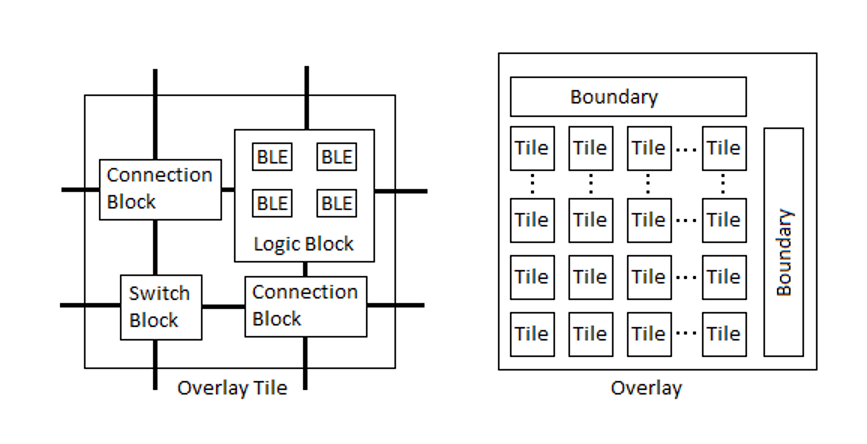
\includegraphics[scale=0.7]{overlay.png}

The above schematic illustrates the organization of both the structure of a single tile in the overlay, as well as the overlay itself.
Each tile is composed of 3 different types of modules: logic block, connection block, and switch block.
The tiles are then tessellated together into the overlay, with extra boundaries added on two sides to make it symmetrical.

At the moment, the logic block, connection block, and switch blocks are all complete. The overlay itself still requires testing and debugging to ensure functionality.

\pagebreak
\section{Resource Usage Per Tile}

\begin{tabular}{|l|l|l|l|l|l|l|}
\hline
\textbf{Bus Width} & \textbf{Logic Block Input} & \textbf{Logic Block Output} & \textbf{SRL/Tile} & \textbf{Tiles/Board} \\ \hline
\hline
2 & 16 & 4 & 160 & 216 \\ \hline
3 & 16 & 4 & 200 & 172 \\ \hline
2 & 24 & 4 & 264 & 130\\ \hline
3 & 24 & 4 & 320 & 108\\ \hline
4 & 24 & 4 & 328 & 105\\ \hline
5 & 24 & 4 & 360 & 96\\ \hline
5 & 12 & 4 & 216 & 160\\ \hline
5 & 16 & 4 & 232 & 148\\ \hline
5 & 20 & 4 & 272 & 127\\ \hline
5 & 16 & 8 & 408 & 84\\ \hline
5 & 20 & 8 & 568 & 60\\ \hline
5 & 24 & 8 & 632 & 54\\ \hline
3 & 24 & 8 & 592 & 58\\ \hline
4 & 24 & 8 & 600 & 57\\ \hline
\end{tabular}

The table above shows the number of shift registers used in a single tile in the overlay for different parameters chosen. The numbers were acquired from Xilinx Xpower Analyzer after a single tile with the specified parameter was implemented.

The numbers have a large range depending on the parameter settings, with the most significant parameter being the number of outputs (basic logic elements) per logic block. The board we're using contains approximately 35,000 shift registers of the appropriate type. This means that we can fit only around 200 tiles on a single board with the lowest parameter settings. This number is significantly less than our initial goal, but still enough to make the project a successful proof-of-concept. If we have enough time after the overlay and the bitstream are debugged and tested, we may look to reducing the number of SRL/tile used to boost the maximum possible size of the overlay.


\end{appendices}

\end{document}


